\section*{Results}

\subsection*{1. Two-trait outcomes}








\begin{figure}[ht!]
\centering
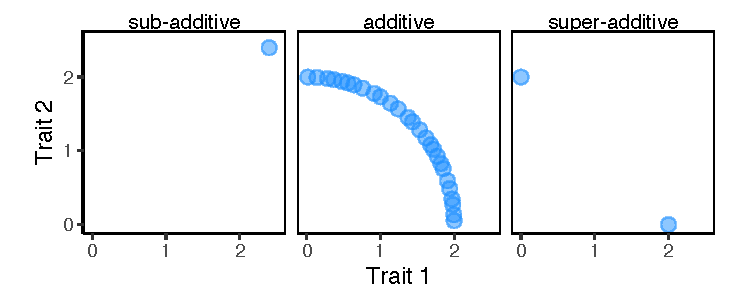
\includegraphics{1-outcomes_q2.pdf}
\caption{Unique trait values for surviving species, for tradeoffs
    being sub-additive, additive, or super-additive.}
\label{fig:two-trait-outcomes}
\end{figure}



With three traits, we first generated the 3 $\eta$ magnitudes from a
uniform distribution from 0.1 to 0.4.
The values we ended up with were
$\eta_1 = 0.207$, $\eta_2 = 0.190$, and $\eta_3 = 0.257$.
We then simulated communities of 100 species, each with random starting
trait values ($\sim \text{N}(0, 2)$, truncated to be $\ge 0$).
We did this 24 times for each of the 27 permutations of
$\eta_1$, $\eta_2$, and $\eta_3$ being negative, zero, or positive.
Because we were only interested in the possible trait values for surviving
species, we set $d = 0.1$ (non-conflicting evolution) so that many species
survived and surveyed the trait space more effectively.
We recorded the trait values of the surviving species.


This resulted in a number of outcomes (Figure \ref{fig:two-trait-outcomes}).
When at least one combination was sub-additive, only one set of trait
values were present in surviving species.
What those trait values were depended on the exact combination.
With all sub-additive combinations, all three traits were maximized.
The six other permutations of $\ge 2$ sub-additive combinations varied but
all had high values of $\eta_2$ and usually had high values of $\eta_3$.
With only one sub-additive combination, the combination that was sub-additive
determined which of the three trait states the surviving species possessed.


We observed alternative trait states only when no trait combinations
were sub-additive.
When all combinations were super-additive, there were three alternative
trait states: one for each trait being maximized while the others
equaled zero.
With two super-additive and one neutral combinations, species traits were
along a neutrally stable quarter-ring along one axis.
With one super-additive and two neutral combinations, species traits were
along a neutrally stable half-ring along two axes.
Traits existed along a neutrally stable three-dimensional shell when all
traits were neutral.



\textbf{NOTE:} When $d$ is large enough ($d = 0.9$ does it for these parameter values),
you can get additional trait outcomes.
In some cases, it adds 1 or 2 additional trait state(s), but in the case
of 1 sub-additive, 1 neutral, and 1 super-additive trait (i.e., "1 of each"),
it allows for many possibilities:
anywhere on a sub-section of the neutral ring (like
the "2 super, 1 neutral" scenario, but even more reduced).
The species that exist at these additional trait states
have at least slightly lower densities than the others at the trait state
that exists when $d = 0.1$.
Is this interesting or likely an artifact?



\subsection*{2. Conditional coexistence}

\begin{figure}[ht!]
\centering
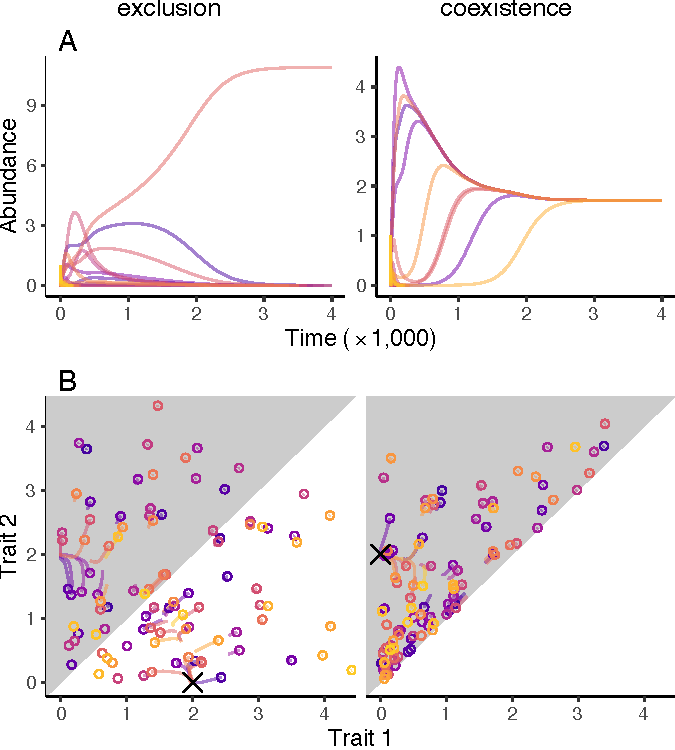
\includegraphics{2-cond_coexist.pdf}
\caption{Two simulations illustrating conditional coexistence for one
    conflicting and one non-conflicting trait.
    The left panels show exclusion, whereas the right two show
    conditional coexistence.
    In the top two panels, each line is for a particular species.
    In the bottom two panels, circles show starting trait values,
    and lines show trajectories through trait space through time.
    Xs show the trait values for surviving species.
    The gray area is the basin of attraction for the
    non-conflicting trait.}
\label{fig:cond-coexist}
\end{figure}


\subsection*{3. Coexistence}


\begin{figure}[ht!]
\centering
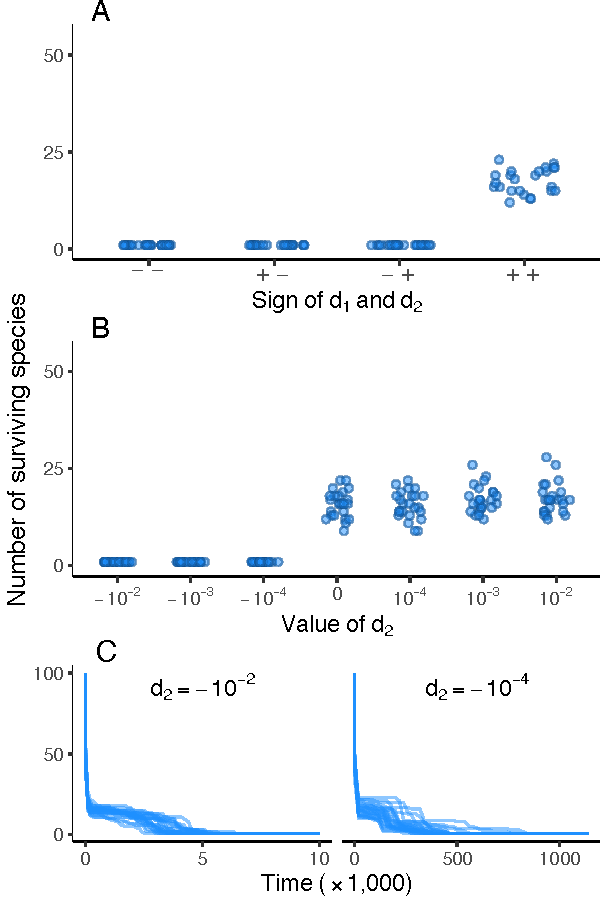
\includegraphics{3-coexist.pdf}
\caption{Number of surviving species for
    (A) all permutations of two traits being conflicting (``$-$'')
    or non-conflicting (``$+$''),
    (B) varying values of $d_2$ when $d_1$ is kept positive
    (i.e., trait 1 is kept non-conflicting), and
    (C) surviving species through time with $d_2 = -10^{-2}$ and
    $d_2 = -10^{-4}$.}
\label{fig:coexist}
\end{figure}


To assess how conflicting and non-conflicting evolution leads to coexistence,
we conducted similar simulations to the previous section, for each of the
8 permutations of the three traits' evolution being conflicting or
non-conflicting (i.e., $d < 0$ or $d > 0$, respectively).
The magnitudes of the $d$ values used for these simulations were generated as
$\log(d) \sim \text{U}(-6, -2)$.
The values we ended up with were % $d_1 = `r sprintf("%#.3g", ds[1])`$,
% }$d_2 = `r sprintf("%#.3f", ds[2])`$, and
% $d_3 = `r sprintf("%#.3g", ds[3])`$.
...
% 
We recorded the number of species coexisting at the end of each repetition.
We also did another set of simulations where the first two traits were kept
non-conflicting ($d_1 = d_2 = 0.1$), while the value of $d_3$ varied
from $-10^{-2}$ to $10^{-2}$.
We used $\eta_1 = \eta_2 = \eta_3 = 0.2$ for all simulations here.

The first set of simulations shows that
coexistence occurs only when evolution for all traits is non-conflicting
(Figure \ref{fig:coexist}A).
From the second set of simulations, we see that a value of 0 for $d_3$
appears to represent a bifurcation with respect to whether
coexistence can occur (Figure \ref{fig:coexist}B).
Even slightly negative values of $d_3$ cause exclusion to occur, although
a less-negative $d_3$ causes the exclusions to happen much more slowly
(Figure \ref{fig:coexist}C).






\subsection*{4. Conditional coexistence}

In the simulations above, we found that with random starting trait values,
only one trait being conflicting causes total exclusion to occur.
In this section, I show that non-random patterns of starting trait values
can result in coexistence.
Specifically, coexistence will occur despite a conflicting trait if all
species start outside the basin of attraction for the state at which
the conflicting trait is maximized.
In these simulations, the first trait is conflicting and the others
are non-conflicting.
We start the communities with 100 species.
One simulation gives these species random trait values
($\mathbf{V} \sim |\text{N}(0,2)|$).
In the other simulation, we forced starting trait 1 to be less than trait 2
for all species ($\mathbf{v}_1 \sim |\text{N}(0,2)|$ and
$\mathbf{v}_2 \sim \text{U}(0, \mathbf{v}_2)$).
This kept all species outside the basin of attraction for the conflicting trait.
We kept trait 3 at zero for all simulations, for the reasons outlined in
the last section.
We kept track of abundances and trait values through time for all species.



When simulations started with a population whose trait values were all in the
basin of attraction for a non-conflicting trait, species evolve towards the
adaptive peak for the non-conflicting trait---and can coexist with one another
(Figure 4).
When the population starts with some species in the basin of attraction for
the conflicting trait, those species evolve towards that adaptive peak, and
the one that reaches the peak first excludes all other species.
